\documentclass{article}

\usepackage{amsmath}
\usepackage{graphicx}
\usepackage{float}
\usepackage[font=scriptsize,labelfont=bf]{caption}
\usepackage{bm}
\usepackage{arydshln}
\usepackage[dvipsnames]{xcolor}
\usepackage{amsfonts}
\usepackage[textwidth=450pt]{geometry}
\usepackage{nicematrix}

\definecolor{grayII}{gray}{0.3}

\begin{document}

We want to find out what a guitar string with variable mass density would sound like. Our model is based on \eqref{we}: a 1D wave equation with variable speed of sound:

\begin{equation}\label{we}
\boxed{\frac{1}{c(x)^2}\frac{\partial^2 \Phi}{\partial t^2}=\frac{\partial^2 \Phi}{\partial x^2}.}
\end{equation}

From the mathematical theory of partial differential equations (EDPs), we know that we need both boundary and initial conditions to get a unique solution. For a guitar string, we impose:

\begin{equation}\label{cwe}
\left\{\begin{array}{cc}
\displaystyle\frac{1}{c(x)^2}\frac{\partial^2 \Phi}{\partial t^2}=\frac{\partial^2 \Phi}{\partial x^2},&0<x<L,\text{ }t>0\\
\text{ }&\text{ }\\
\displaystyle \Phi(t,0)=\Phi(t,L)=0&\text{ }\\
\text{ }&\text{ }\\
\displaystyle\Phi(0,x)=f(x)&\text{ }\\
\text{ }&\text{ }\\
\displaystyle\frac{\partial \Phi}{\partial t}(0,x)=g(x)&\text{ }
\end{array}\right.,
\end{equation}
where $L$ is the length of the string and $f(x)$ and $g(x)$ are functions representing the shape and the velocity of the string, respectively, upon being plucked.

For our purposes, it is more convenient to work with first order equations in time. Define $\Pi(t,x)\equiv\displaystyle\frac{\partial \Phi}{\partial t}$. The problem \eqref{cwe} is then translated into:

\begin{equation}\label{cweII}
\left\{\begin{array}{cc}
\displaystyle\frac{\partial \Phi}{\partial t}=\Pi&0<x<L,\text{ }t>0\\
\text{ }&\text{ }\\
\displaystyle\frac{\partial \Pi}{\partial t}=c(x)^2\frac{\partial^2 \Phi}{\partial x^2}&\text{ }\\
\text{ }&\text{ }\\
\displaystyle \Phi(t,0)=\Phi(t,L)=0&\text{ }\\
\text{ }&\text{ }\\
\displaystyle\Phi(0,x)=f(x)&\text{ }\\
\text{ }&\text{ }\\
\displaystyle\Pi(0,x)=g(x)&\text{ }
\end{array}\right..
\end{equation}


\section{Finite Differences Method}

In the finite differences approach, we need to discretize the domain into a grid of points. For simplicity, we choose a regular grid, as shown in figure \ref{fig1}.

\begin{figure}[H]
\centering
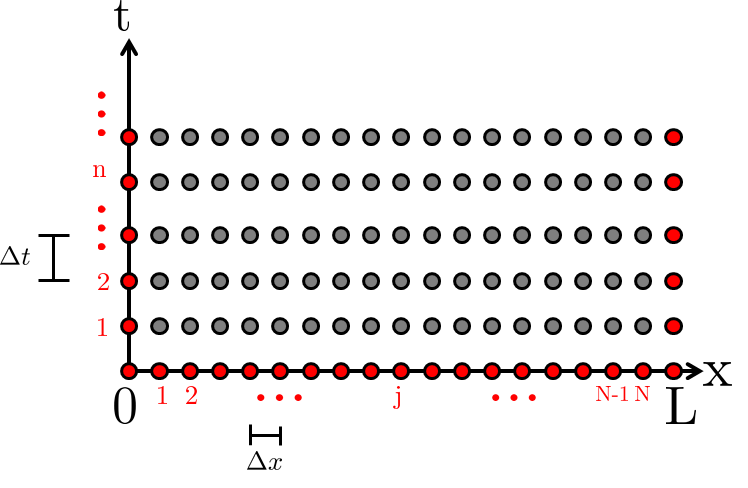
\includegraphics[width=0.8\textwidth]{figgrid}
\caption{\label{fig1}Spacetime discretization grid to be used in the numerical solution of the problem. We show in red the boundary of the domain where the problem is defined. The labeling is chosen so that there are $N$ spatial points \textit{not on the boundary for a given time step}.}
\end{figure}

As can be seen in figure \ref{fig1}, each point in the grid $(t_n,x_j)$ is labeled by a spatial index $j=0,1,..., N+1$ and a temporal index $n=0,1,...$. The points are separated from each other by both a spatial step $\Delta x$ and a time step $\Delta t$. Our unknown functions $\Phi(t,x)$ and $\Pi(t,x)$ can then be evaluated on a specific point $(t_n,x_j)$; we define $\Phi(t_n,x_j)\equiv \Phi^n_j$ and $\Pi(t_n,x_j)\equiv \Pi^n_j$.

Now, we know that, using Taylor expansions, we can aproximate derivatives on a grid. For example, the following is true \textit{if the spatial grid is regular}:

\begin{equation}\label{te}
\left.\frac{\partial^2 \Phi}{\partial x^2}\right|_{(t_n,x_j)}\approx\frac{\Phi^n_{j+1}-2\Phi^n_j+\Phi^n_{j-1}}{\Delta x^2},
\end{equation}
as a second-order approximation for the laplacian operator. Let us then choose a general time step $t_n$, $n\neq0$, and apply the equations of motion for every point $x_j$ \textit{not on the boundary}:

\begin{equation}\label{discr}
\left\{\begin{array}{cc}
\displaystyle\left(\frac{\partial\Phi}{\partial t}\right)^n_j=\Pi^n_j&j=1,2,...,N,\text{ }n=1,2,...\\
\text{ }&\text{ }\\
\displaystyle\left(\frac{\partial \Pi}{\partial t}\right)^n_j=\left(c^n_j\right)^2\left(\frac{\Phi^n_{j+1}-2\Phi^n_j+\Phi^n_{j-1}}{\Delta x^2}\right)&\text{ }
\end{array}\right..
\end{equation}

The reason we apply the functions only on points not on the boundary is very simple: strictly speaking, differential equations are not defined on it. The boundary conditions, however, fix the values of the unknowns beforehand.

For a given time step $t_n$, $n\neq0$, we can interpret \eqref{discr} as a system of equations for the components of the vector:

\begin{equation}\label{Y}
\bm{Y}^n\equiv\left[\begin{array}{c}
\Phi^n_1\\
\Phi^n_2\\
\vdots\\
\Phi^n_{N-1}\\
\Phi^n_N\\
\hdashline
\Pi^n_1\\
\Pi^n_2\\
\vdots\\
\Pi^n_{N-1}\\
\Pi^n_N\\
\end{array}\right].
\end{equation}

Indeed, because the wave equation is linear, it is convenient to condense the unknowns into a big vector. We can then write the right-hand side of \eqref{discr} as $\bm{M}^n\cdot\bm{Y}^n$ for a suitable matrix $\bm{M}^n$ that depends only on the parameters of the problem (in the present case, the speed of sound function $c(x)$).

However, one must be careful in constructing the matrix $\bm{M}^n$. Remember that the boundary values $\Phi^n_0$, $\Phi^n_{N+1}$, $\Pi^n_0$ and $\Pi^n_{N+1}$ do not enter $\bm{Y}^n$ as they are not unknowns. In order to see this clearly, take for example $j=1$ and $j=2$ in the second set of equations in \eqref{discr}:

\begin{equation}\label{calma}
\left\{\begin{array}{c}
\displaystyle\left(\frac{\partial \Pi}{\partial t}\right)^n_1=\textcolor{grayII}{-2\frac{\left(c^n_1\right)^2}{\Delta x^2}}\Phi^n_1+\textcolor{grayII}{\frac{\left(c^n_1\right)^2}{\Delta x^2}}\Phi^n_2+\textcolor{Red}{\frac{\left(c^n_1\right)^2}{\Delta x^2}\Phi^n_{0}}\\
\text{ }\\
\displaystyle\left(\frac{\partial \Pi}{\partial t}\right)^n_2=\textcolor{grayII}{\frac{\left(c^n_2\right)^2}{\Delta x^2}}\Phi^n_1-\textcolor{grayII}{2\frac{\left(c^n_2\right)^2}{\Delta x^2}}\Phi^n_2+\textcolor{grayII}{\frac{\left(c^n_2\right)^2}{\Delta x^2}}\Phi^n_3
\end{array}\right..
\end{equation}

In \eqref{calma}, we use the same color scheme as in figure \ref{fig1}: gray indicates points inside the open domain and red indicates points on its boundary. Something similar happens for $j=N-1$ and $j=N$:

\begin{equation}\label{calmaII}
\left\{\begin{array}{c}
\displaystyle\left(\frac{\partial \Pi}{\partial t}\right)^n_{N-1}=\textcolor{grayII}{\frac{\left(c^n_{N-1}\right)^2}{\Delta x^2}}\Phi^n_{N-2}-\textcolor{grayII}{2\frac{\left(c^n_{N-1}\right)^2}{\Delta x^2}}\Phi^n_{N-1}+\textcolor{grayII}{\frac{\left(c^n_{N-1}\right)^2}{\Delta x^2}}\Phi^n_N\\
\text{ }\\
\displaystyle\left(\frac{\partial \Pi}{\partial t}\right)^n_N=\textcolor{grayII}{\frac{\left(c^n_N\right)^2}{\Delta x^2}}\Phi^n_{N-1}-\textcolor{grayII}{2\frac{\left(c^n_N\right)^2}{\Delta x^2}}\Phi^n_N+\textcolor{Red}{\frac{\left(c^n_N\right)^2}{\Delta x^2}\Phi^n_{N+1}}
\end{array}\right..
\end{equation}

Therefore, if we want to write the right-hand side of the second group of equations in \eqref{discr} as a linear system on the variables $(\Phi^n_1,\Phi^n_2,...,\Phi^n_{N-1},\Phi^n_N)$, the red terms in \eqref{calma} and \eqref{calmaII} have to be written as a non-homogeneous contribution. In other words, we will have $\textcolor{grayII}{A}\cdot(\Phi^n_1,\Phi^n_2,...,\Phi^n_{N-1},\Phi^n_N)+\textcolor{Red}{b}$ for given $\textcolor{grayII}{A}$ and $\textcolor{Red}{b}$. In particular, it is clear that $\textcolor{grayII}{A}$ is a tridiagonal matrix and the only non-zero entries of $\textcolor{Red}{b}$ are its first and last components.

We still have to consider the first set of equations in \eqref{discr}. It poses no problem though, since only the same points $j$ appear. Therefore, equations \eqref{discr} can finally be written:

\begin{equation}\label{syst}
\left[\begin{array}{c}
\displaystyle\left(\frac{\partial \Phi}{\partial t}\right)^n_1\\
\vdots\\
\displaystyle\left(\frac{\partial \Phi}{\partial t}\right)^n_N\\
\text{ }\\
\hdashline\\
\displaystyle\left(\frac{\partial \Pi}{\partial t}\right)^n_1\\
\vdots\\
\displaystyle\left(\frac{\partial \Pi}{\partial t}\right)^n_N
\end{array}\right]=\textcolor{grayII}{\left[\begin{array}{ccccc:ccccc}
 & & & & & & & & & \\
 & & & & & & & & & \\
 & &\displaystyle\mathbb{O}& & & & &\displaystyle\mathbb{I}& & \\
 & & & & & & & & & \\
 & & & & & & & & & \\
\hdashline
 \ddots&\ddots& & & & & & & & \\
\ddots&\ddots&\ddots& & & & & & & \\
 &\ddots&\ddots&\ddots& & & &\displaystyle\mathbb{O}& & \\
 & &\ddots&\ddots&\ddots& & & & & \\
 & & &\ddots&\ddots& & & & & 
\end{array}\right]} \left[\begin{array}{c}\displaystyle\Phi^n_1\\\vdots\\\displaystyle\Phi^n_N\\\text{ }\\\hdashline\\\displaystyle\Pi^n_1\\\vdots\\\displaystyle\Pi^n_N\end{array}\right]+\textcolor{Red}{\left[\begin{array}{c}0\\\vdots\\0\\\hdashline\\\displaystyle\frac{(c^n_1)^2}{\Delta x^2}\Phi^n_0\\\text{ }\\0\\\vdots\\0\\\text{ }\\\displaystyle\frac{(c^n_N)^2}{\Delta x^2}\Phi^n_{N+1}\end{array}\right]},
\end{equation}
where $\mathbb{O}$ and $\mathbb{I}$ represent the null matrix and the indentity matrix, respectively. The tridiagonal block is the matrix $\textcolor{grayII}{A}$ discussed before. Defining $\textcolor{Red}{\bm{B}}$ as the boundary condition vector, we can then write:

\begin{equation}\label{cond}
\left[\begin{array}{c}
\displaystyle\left(\frac{\partial \Phi}{\partial t}\right)^n_1\\
\vdots\\
\displaystyle\left(\frac{\partial \Phi}{\partial t}\right)^n_N\\
\text{ }\\
\hdashline\\
\displaystyle\left(\frac{\partial \Pi}{\partial t}\right)^n_1\\
\vdots\\
\displaystyle\left(\frac{\partial \Pi}{\partial t}\right)^n_N
\end{array}\right]=\textcolor{grayII}{\bm{M^n}}\cdot \bm{Y^n}+\textcolor{Red}{B^n}\equiv \bm{F^n}(\bm{Y^n})
\end{equation}

Only one time step $t_n$, $n\neq0$ has been dealt with so far. Now, we want to evolve our initial conditions in time using \eqref{cond}.

\subsection{Explicit Euler Method}

We can again make use of Taylor expansions. Now we do it in the time coordinate instead. The following is true:

\begin{equation}\label{ttaylor}
\bm{Y^{n}}\equiv\left.\bm{Y}\right|_{t_n}\approx\left.\bm{Y}\right|_{t_{n-1}}+\left.\frac{d \bm{Y}}{d t}\right|_{t_{n-1}}\Delta t.
\end{equation}
But $\displaystyle\frac{d \bm{Y}}{d t}$ is given by \eqref{cond}. Therefore:

\begin{equation}\label{eeuler}
\boxed{\bm{Y^{n}}\approx\bm{Y^{n-1}}+\bm{F^{n-1}}(\bm{Y^{n-1}})\Delta t, \text{ }n=1,2,...}
\end{equation}

This is the \textit{explicit Euler method}: we can find the values of the unknowns on a chosen time step using only their values on the previous time step. Notice that, from \eqref{cond}, the function $\bm{F^n}$ \textit{already incorporates the boundary conditions} and, thus, the evolution takes them into account. Furthermore, $\bm{F^n}$ depends on the time step itself, so that in general we have to build a new matrix for each step. Nevertheless, our problem is a little bit simpler: because neither the speed of sound nor the boundary conditions are functions of time, the evolution matrix coming from $\bm{F}$ is the same for all iterations. We then only need to build one matrix and keep applying it to the each time step vector. 

\subsection{Implicit Euler Method}

Explicit methods have a caveat: they usually amplify numerical errors at each iteration, leading to an unphysical growing solution. This can be dealt with by introducing numerical dissipation terms into the wave equation itself. Alternatively, one can try using implicit methods instead.

Implicit methods are also based on Taylor expansions. In \eqref{ttaylor}, we used a Taylor series to approximate the value of the solution vector at $t_n=t_{n-1}+\Delta t$ from its value at $t_{n-1}$. The opposite also works. Given $\bm{Y^n}=\left.\bm{Y}\right|_{t_n}$, we can aproximate $\bm{Y}^{n-1}=\left.\bm{Y}\right|_{t_{n-1}}=\left.\bm{Y}\right|_{t_n-\Delta t}$ by:

\begin{equation}\label{ttaylorimp}
\bm{Y^{n-1}}\approx\left.\bm{Y}\right|_{t_{n}}-\left.\frac{d \bm{Y}}{d t}\right|_{t_{n}}\Delta t.
\end{equation}
Again, from \eqref{cond}, we can write:

\begin{equation}\label{eeulerimp}
\boxed{\bm{Y^{n}}-\bm{F^{n}}(\bm{Y^n})\Delta t\approx\bm{Y^{n-1}}, \text{ }n=1,2,...}
\end{equation}

However, we do not know $\bm{Y^n}$; this is exactly what we want to find from a given $\bm{Y^{n-1}}$. Equation \eqref{eeulerimp}, then, involves calculating the inverse of the matrix $\bm{\mathbb{I}}-\textcolor{grayII}{\bm{M^n}}$ for each iteration. Once again, our guitar string setting is simpler: we only need to calculate this inverse matrix once, since neither the speed of sound function nor the boundary conditions depend on time.

\subsection{Explicit Runge-Kutta Method}
Involves calculating $\bm{F}$ in ``virtual'' points between $t_{n-1}$ e $t_{n}$.

\subsection{Implicit Runge-Kutta Method}
Same thing but implicit.

\subsection{Crank-Nicolson Method}
Average between explicit and implicit Euler.
\end{document}




